\documentclass[12pt,a4paper,twoside,openany]{book}
\usepackage{graphicx}
\usepackage{setspace} % espaciado doble para texto, simple para pies de página, subtítulos, etc.
\usepackage{natbib} % sustituto de 'hypernat' que funciona en Windows.
\usepackage[spanish]{babel}
\usepackage[utf8]{inputenc}
\usepackage{color}
\usepackage{hhline} % estilos extendidos para tablas
\usepackage{multirow}
\usepackage{subfigure}
\usepackage{acronym}
\usepackage{hyperref}
\usepackage{amsmath,amssymb}
\usepackage{fancyhdr}
\usepackage{epsfig, amsmath}
\usepackage{algorithm}
\usepackage{algorithmic}
\usepackage[T1]{fontenc}
\usepackage{lmodern}
\usepackage{microtype}
\usepackage{tabularx}
\usepackage{longtable}
\usepackage{array}

\let\cleardoublepage\clearpage

% configuraciones generales
\hypersetup{
linktocpage=true,
colorlinks=true,
linkcolor=blue,
citecolor=blue,
}
\definecolor{Hgray}{gray}{0.6}

\newenvironment{definition}[1][Definición]{\begin{trivlist}
\item[\hskip \labelsep {\bfseries #1}]}{\end{trivlist}}

\setlength{\topmargin}{0cm}
\setlength{\textheight}{23cm}
\setlength{\textwidth}{17cm}
\setlength{\oddsidemargin}{0cm}
\setlength{\evensidemargin}{0cm}
\setlength{\headheight}{1cm}

% indica que las 'sub-sub-secciones' están numeradas y aparecen en el índice
\setcounter{secnumdepth}{3}
\setcounter{tocdepth}{2}

% configuraciones para código
\renewcommand{\algorithmicrequire}{\textbf{Entrada:}}
\renewcommand{\algorithmicensure}{\textbf{Salida:}}

%%%%%%%%%%%%
% DOCUMENTO %
%%%%%%%%%%%%
\begin{document}

\setcounter{section}{0} % Restablece el contador de sección a 0 al inicio del documento
\renewcommand{\thesection}{\arabic{section}} % Cambia el esquema de numeración de sección

\pagenumbering{arabic}

\hypersetup{pageanchor=true}

% portada
\newpage
\thispagestyle{empty}

\baselineskip 2em

%\vspace*{1cm}

\centerline{
\includegraphics[width=0.6\textwidth]{images/UOC-logo}}
\begin{center}
\textsc{Universitat Oberta de Catalunya (UOC) \\
 Máster Universitario en Ciencia de Datos (\textit{Data Science})\\}

%\centerline {\pic{UOC}{4cm}}

\vspace*{1.5cm}

\textsc{\Large TRABAJO FINAL DE MÁSTER}

\vspace*{0.5cm}

\textsc{\large Área: Reinforced Learning}


%\textbf{\Huge VirtualTechLab Model: }

\vspace*{2.0cm}

\textbf{\Large Impacto de la complejidad de las observaciones en el rendimiento de algoritmos de Aprendizaje por Refuerzo en un entorno Pacman}

\vspace{2.5cm}
\baselineskip 1em

\baselineskip 2em
-----------------------------------------------------------------------------\\
Autor:      Alejandro Suau Ruiz\\
Tutor:      Marc Borras Camarasa\\
Profesor:   David Masip Rodó\\
-----------------------------------------------------------------------------\\
\vspace*{1.5cm}
Palma de Mallorca, \today

\end{center}

\newpage
\pagestyle{empty}
\hfill

\newpage
% resumen
\hypersetup{pageanchor=false}
\pagenumbering{roman} 
\setcounter{page}{1} 
\pagestyle{plain}

%%%%%%%%%%%%%%%%
%%% CREDITOS %%%
%%%%%%%%%%%%%%%%
\chapter*{Créditos/Copyright}

Una página con la especificación de créditos/copyright para el proyecto (ya sea aplicación por un lado y documentación por el otro, o unificadamente), así como la del uso de marcas, productos o servicios de terceros (incluidos códigos fuente). Si una persona diferente al autor colaboró en el proyecto, tiene que quedar explicitada su identidad y qué hizo.

A continuación se ejemplifica el caso más habitual, aunque se puede modificar por cualquier otra alternativa:

\vspace{1cm}

\begin{figure}[ht]
    \centering
	
\includegraphics[scale=1]{images/license.png}
\end{figure}

Esta obra está sujeta a una licencia de Reconocimiento -  NoComercial - SinObraDerivada

\href{https://creativecommons.org/licenses/by-nc-nd/3.0/es/}{3.0 España de CreativeCommons}.

%%%%%%%%%%%%%
%%% FICHA %%%
%%%%%%%%%%%%%
\chapter*{FICHA DEL TRABAJO FINAL}

\begin{table}[ht]
	\centering{}
	\renewcommand{\arraystretch}{2}
	\begin{tabular}{r | l}
		\hline
		Título del trabajo: & Impacto de la complejidad de las observaciones en el rendimiento de algoritmos de Aprendizaje por Refuerzo en un entorno Pacman\\
		\hline
        Nombre del autor: & Alejandro Suau Ruiz\\
		\hline
        Nombre del colaborador/a docente: & Marc Borras Camarasa\\
		\hline
        Nombre del PRA: & David Masip Rodó\\
		\hline
        Fecha de entrega (mm/aaaa): & 01/2026\\
		\hline
        Titulación o programa: & Máster Universitario de Data Science\\
		\hline
        Área del Trabajo Final: & Reinforced Learning\\
		\hline
        Idioma del trabajo: & Español\\
		\hline
        Palabras clave & Aprendizaje por refuerzo, Complejidad del estado, Pacman\\
		\hline
	\end{tabular}
\end{table}

%%%%%%%%%%%%%%%%%%%
%%% DEDICATORIA %%%
%%%%%%%%%%%%%%%%%%%
\chapter*{Dedicatoria/Cita}

Breves palabras de dedicatoria y/o una cita.

%%%%%%%%%%%%%%%%%%%
%%% Agradecimientos %%%
%%%%%%%%%%%%%%%%%%%
\chapter*{Agradecimientos}

Si se considera oportuno, mencionar a las personas, empresas o instituciones que hayan contribuido en la realización de este proyecto.

%%%%%%%%%%%%%%%%
%%% ABSTRACT%%%
%%%%%%%%%%%%%%%%
\chapter*{Abstract}
\addcontentsline{toc}{chapter}{Abstract}

\onehalfspacing

This work investigates how the complexity of state representation affects the performance of reinforcement learning algorithms in a simplified Pacman environment. The central idea is that an agent’s success depends not only on the algorithm itself but also on the quality and richness of the information it receives from the environment. To analyze this, we designed a set of progressively more complex observation spaces, ranging from the basic positions of the player and the ghost to configurations that include the presence and duration of power-ups and the distribution of coins across quadrants.
Experiments were carried out using widely adopted algorithms such as PPO, A2C, and DQN, implemented with the Stable-Baselines3 library. Controlled training with different random seeds and consistent performance metrics allowed us to compare both learning speed and the stability of the learned policies.
The results show that increasing state complexity does not always lead to better performance: in some cases, the additional information introduces noise and hinders convergence. However, for specific configurations, the agent was able to exploit the extra information to achieve more robust behavior.
In conclusion, the project highlights the importance of observation design in the success of reinforcement learning agents, stressing the need to balance simplicity and expressiveness depending on the task and the chosen algorithm.

\vspace{1.5cm}

\textbf{Keywords}: Reinforcement learning, State complexity, Pacman, Stable-Baselines3, Gymnasium

%%%%%%%%%%%%%%%%
%%% RESUMEN    %%%
%%%%%%%%%%%%%%%%

\chapter*{Resumen}
\addcontentsline{toc}{chapter}{Resumen}

\onehalfspacing

Este trabajo explora cómo la complejidad de la representación del estado influye en el rendimiento de los algoritmos de aprendizaje por refuerzo en un entorno simplificado de Pacman. Partimos de la premisa de que un agente no aprende únicamente por el algoritmo empleado, sino también por la calidad y la riqueza de la información que percibe del entorno. Para analizarlo, hemos diseñado un conjunto de observaciones progresivamente más complejas, desde la posición básica de jugador y fantasma, hasta configuraciones que incluyen la presencia y duración de comodines o la distribución de monedas por cuadrantes.
La experimentación se ha llevado a cabo con algoritmos ampliamente utilizados, como PPO, A2C y DQN, implementados con la librería Stable-Baselines3. Se han realizado entrenamientos controlados con semillas distintas y métricas de rendimiento homogéneas, lo que ha permitido comparar tanto la velocidad de aprendizaje como la estabilidad de las políticas aprendidas.
Los resultados muestran que un aumento en la complejidad del estado no garantiza siempre un mejor desempeño: en ciertos casos, la mayor riqueza de información introduce ruido y dificulta la convergencia. Sin embargo, para determinadas configuraciones el agente logra aprovechar la información adicional y alcanzar un comportamiento más robusto.
En conclusión, el proyecto confirma la relevancia del diseño de observaciones en el éxito de un agente de aprendizaje por refuerzo, subrayando la necesidad de equilibrar simplicidad y expresividad en función del objetivo y del algoritmo empleado.


\vspace{1.5cm}

\textbf{Palabras clave}: Aprendizaje por refuerzo, Complejidad del estado, Pacman, Stable-Baselines3, Gymnasium
\newpage

\pagestyle{fancy}
\renewcommand{\chaptermark}[1]{ \markboth{#1}{}}
\renewcommand{\sectionmark}[1]{\markright{ \thesection.\ #1}}
\lhead[\fancyplain{}{\bfseries\thepage}]{\fancyplain{}{\bfseries\rightmark}}
\rhead[\fancyplain{}{\bfseries\leftmark}]{\fancyplain{}{\bfseries\thepage}}
\cfoot{}

% tabla de contenidos
\cleardoublepage
\phantomsection
\addcontentsline{toc}{chapter}{Índice}
\tableofcontents
% lista de figuras
\cleardoublepage
\phantomsection
\addcontentsline{toc}{chapter}{Lista de Figuras}
\listoffigures
% lista de tablas
\cleardoublepage
\phantomsection
\addcontentsline{toc}{chapter}{Lista de Tablas}
\listoftables

\thispagestyle{empty}

\pagenumbering{arabic}

\pagestyle{fancy}
\renewcommand{\chaptermark}[1]{ \markboth{#1}{}}
\renewcommand{\sectionmark}[1]{\markright{ \thesection.\ #1}}
\lhead[\fancyplain{}{\bfseries\thepage}]{\fancyplain{}{\bfseries\rightmark}}
\rhead[\fancyplain{}{\bfseries\leftmark}]{\fancyplain{}{\bfseries\thepage}}
\cfoot{}

\onehalfspacing

% capítulos del documento
\section{Introducción}

El \textit{Aprendizaje por Refuerzo} (\textit{Reinforcement Learning}, RL) se ha consolidado como una de las ramas más activas y prometedoras del aprendizaje automático. A diferencia del aprendizaje supervisado, en el que el modelo aprende a partir de ejemplos etiquetados, el RL se fundamenta en la interacción continua de un agente con un entorno, buscando maximizar una recompensa acumulada. Este paradigma ha permitido resolver problemas complejos de toma de decisiones secuenciales en campos tan diversos como la robótica, los videojuegos, la gestión de recursos o la conducción autónoma.

En los últimos años, la combinación del RL con redes neuronales profundas —conocida como \textit{Deep Reinforcement Learning} (DRL)— ha supuesto un gran avance, al permitir que los agentes aprendan directamente a partir de observaciones de alta dimensión. Algoritmos como \textit{Deep Q-Network} (DQN) o \textit{Proximal Policy Optimization} (PPO) han demostrado su eficacia en entornos complejos como Atari o MuJoCo, donde el espacio de estados y de acciones puede ser extremadamente amplio.

Sin embargo, el rendimiento de un agente no depende únicamente del algoritmo de aprendizaje empleado, sino también de la representación del estado con la que percibe el entorno. En otras palabras, la complejidad de la observación influye directamente en la capacidad del agente para generalizar, explorar y aprender políticas efectivas. Representaciones demasiado simples pueden limitar el aprendizaje al ocultar información relevante, mientras que representaciones demasiado complejas pueden ralentizar la convergencia y requerir una mayor capacidad de red o una exploración más prolongada.

En este Trabajo Fin de Máster se analiza precisamente cómo afecta la complejidad del estado observado al rendimiento del agente en un entorno controlado. Para ello, se ha desarrollado un entorno propio denominado \textit{SimplePacmanEnv}, inspirado en el clásico juego \textit{Pac-Man}, pero adaptado para experimentos de RL. Este entorno, implementado con \textit{Gymnasium} y \textit{Stable-Baselines3}, permite configurar diferentes niveles de complejidad en la observación —desde representaciones mínimas (solo posiciones del jugador y el fantasma) hasta observaciones enriquecidas con información global sobre las monedas o incluso representaciones tipo imagen—, manteniendo constantes la dinámica del entorno y la estructura de recompensas.

Sobre esta base se han entrenado y evaluado tres algoritmos representativos de distintas familias del RL profundo: \textit{Advantage Actor-Critic} (A2C), \textit{Proximal Policy Optimization} (PPO) y \textit{Deep Q-Network} (DQN). El objetivo es cuantificar cómo evoluciona el aprendizaje y el rendimiento final de cada agente en función de la información proporcionada por el entorno, y determinar si existe una relación clara entre la complejidad de la representación del estado y la eficiencia del aprendizaje.

Además, el proyecto incorpora herramientas complementarias como \textit{TensorBoard} para la monitorización en tiempo real del entrenamiento, y el uso de \textit{EvalCallback} para realizar evaluaciones periódicas y registrar automáticamente el mejor modelo alcanzado. Estos mecanismos no solo facilitan el análisis experimental, sino que aportan rigor y reproducibilidad a los resultados obtenidos.

En conjunto, este trabajo busca aportar una visión práctica y experimental sobre la influencia de la observación en entornos de aprendizaje por refuerzo, conectando los fundamentos teóricos con un estudio aplicado y reproducible, y poniendo de manifiesto la importancia del diseño de los estados en la efectividad de los algoritmos de RL.

\begin{figure}[h]
\centering
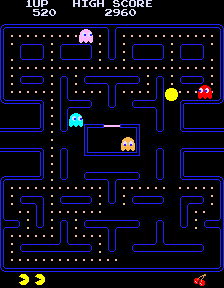
\includegraphics[width=0.5\textwidth]{./figs/image1.png}
\caption{Ejemplo de figura. Será indexada en la “Lista de Figuras”.}
\label{fig:figura_ejemplo}
\end{figure}

\subsection{Contexto y motivación}

\subsubsection{Justificación e interés}
El estudio de la relación entre la complejidad del estado y el rendimiento del agente resulta relevante tanto desde el punto de vista teórico como práctico:

\begin{itemize}
    \item Permite entender la eficiencia y capacidad de generalización de distintos algoritmos (A2C, PPO, DQN) en entornos de distinta dimensionalidad.
    \item Aporta evidencia empírica sobre el compromiso entre simplicidad del modelo y capacidad de representación, tema central en el diseño de entornos y arquitecturas RL.
    \item Facilita la comparación controlada entre configuraciones de observación, aislando el impacto del estado sin alterar dinámicas, recompensas ni mecánicas de juego.
    \item Además, el uso de un entorno propio y reproducible contribuye al valor educativo e investigativo, permitiendo futuras extensiones y análisis.
\end{itemize}

\subsubsection{Motivación personal}

Mi motivación para realizar este proyecto es principalmente educativa e investigativa.
Busco profundizar en el campo del Aprendizaje por Refuerzo, comprendiendo de forma práctica cómo los agentes aprenden a través de la interacción con su entorno y cómo la cantidad de información observada afecta dicho proceso.

El trabajo ha supuesto un ejercicio de integración de conocimientos adquiridos durante el Máster (aprendizaje automático, programación en Python, redes neuronales, y metodologías experimentales) con el objetivo de desarrollar una visión más completa y aplicada del RL.
En última instancia, la meta ha sido explorar, aprender y comprender los fundamentos de la toma de decisiones secuenciales bajo incertidumbre.

\subsection{Objetivos}

\subsubsection{Objetivo principal}

Evaluar cómo el nivel de complejidad del espacio de observación afecta el rendimiento de distintos algoritmos de Aprendizaje por Refuerzo, manteniendo constantes el entorno, las recompensas y la dinámica del juego.

\subsubsection{Objetivos específicos}

\begin{enumerate}
    \item Diseñar e implementar un entorno controlado y parametrizable (basado en Pac-Man) que permita modificar el tipo de observación percibida por el agente.
    \item Entrenar y comparar varios algoritmos de RL (A2C, PPO, DQN) bajo distintos modos de observación.
    \item Analizar métricas de rendimiento (recompensa media, estabilidad, convergencia, tiempo de entrenamiento).
    \item Evaluar la relación entre dimensionalidad del estado y eficiencia del aprendizaje.
    \item Documentar la metodología y resultados, destacando las implicaciones para futuros desarrollos o estudios.
\end{enumerate}

\subsection{Sostenibilidad, diversidad y desafíos ético/sociales}

A continuación se valoran los posibles impactos en materia de sostenibilidad, ética y diversidad.

\paragraph{Sostenibilidad.}
El trabajo se ha realizado íntegramente en un entorno digital y no requiere recursos materiales adicionales, por lo que su impacto medioambiental directo es muy reducido. El único consumo relevante proviene del uso de recursos computacionales durante el entrenamiento de los agentes. Se ha procurado minimizar este impacto mediante el uso de modelos ligeros y tiempos de entrenamiento moderados, evitando configuraciones innecesariamente costosas. Desde una perspectiva positiva, la metodología promueve la eficiencia en la experimentación mediante la reutilización de entornos y scripts reproducibles, contribuyendo así a un uso más sostenible de los recursos de investigación. El proyecto no se ve afectado por ninguna normativa específica en materia medioambiental ni tiene relación directa con los Objetivos de Desarrollo Sostenible (ODS), más allá de fomentar el desarrollo de tecnologías digitales eficientes y abiertas.

\paragraph{Comportamiento ético y responsabilidad social.}
El proyecto no involucra datos personales, información sensible ni toma de decisiones sobre personas o colectivos. Su propósito es exclusivamente académico y experimental. Se han seguido principios de transparencia y reproducibilidad, haciendo uso de bibliotecas abiertas como \textit{Stable-Baselines3} y \textit{Gymnasium}, lo que garantiza la trazabilidad del código y los resultados. En este sentido, el trabajo se alinea con los principios deontológicos de la ingeniería informática, promoviendo la investigación responsable y el acceso abierto al conocimiento. No se identifican impactos negativos sobre el empleo ni sobre aspectos legales o de seguridad.

\paragraph{Diversidad, género y derechos humanos.}
El contenido técnico del trabajo no tiene incidencia directa en cuestiones de género, diversidad o derechos humanos. Sin embargo, se reconoce la importancia de la diversidad en la investigación en inteligencia artificial y el compromiso con un lenguaje inclusivo y accesible en la documentación y la memoria del proyecto. Asimismo, el entorno desarrollado puede emplearse como herramienta docente o de experimentación, favoreciendo la accesibilidad y la igualdad de oportunidades en la formación en técnicas de aprendizaje por refuerzo.

En conjunto, el proyecto presenta un impacto ético, social y medioambiental neutro o ligeramente positivo, destacando por su orientación a la investigación abierta, la eficiencia computacional y el cumplimiento de buenas prácticas profesionales en el ámbito de la inteligencia artificial.


\subsection{Enfoque y metodología}

El presente trabajo adopta un enfoque experimental y comparativo orientado a analizar la influencia de la complejidad del estado sobre el rendimiento de los algoritmos de Aprendizaje por Refuerzo (RL).

\subsubsection{Estrategias consideradas}

Durante la fase inicial del proyecto se evaluaron tres posibles enfoques:

\begin{enumerate}
	\item \textbf{Uso de entornos estándar (Gym / Atari):}
Permitiría aprovechar entornos consolidados como CartPole o Breakout. Sin embargo, estos no ofrecen un control granular sobre la estructura del estado, lo que impide aislar experimentalmente el efecto de la observación.
	\item \textbf{Simulación matemática abstracta (MDP sintético):}
Un enfoque más teórico, usando representaciones vectoriales arbitrarias para estudiar el tamaño del espacio de estado. Aunque más simple de implementar, carece de un contexto visual y de dinámica tangible que facilite la interpretación y comparación intuitiva de los resultados.
	\item \textbf{Diseño de un entorno personalizado (Pacman simplificado):}
Este enfoque combina realismo y control. Permite modificar el nivel de información observable manteniendo constantes las reglas y recompensas.
Además, el dominio es familiar y visualmente interpretable, lo que facilita tanto la depuración como la comunicación de los resultados.
\end{enumerate}

\subsubsection{Estrategia seleccionada}

Se eligió la \textbf{tercera estrategia}, basada en el desarrollo de un entorno propio —SimplePacmanEnv— compatible con Gymnasium y Stable-Baselines3.
Esta elección resulta la más adecuada por las siguientes razones:

\begin{itemize}
	\item Permite \textbf{aislar experimentalmente} la variable de interés (la complejidad del estado), manteniendo el resto de factores constantes.
	\item Facilita la \textbf{comparación justa} entre distintos algoritmos de RL bajo las mismas condiciones.
	\item Favorece la \textbf{reproducibilidad y extensibilidad} del experimento (se pueden añadir observaciones o cambiar reglas sin alterar la estructura general).
	\item Proporciona una \textbf{base educativa sólida}, al exigir una comprensión integral del pipeline de RL: diseño de entorno, configuración del agente y análisis de resultados.
\end{itemize}

\section{Planificación del proyecto}

\subsection{Recursos necesarios}

A continuación se detallan los recursos técnicos, de software y humanos requeridos para el desarrollo del proyecto. La selección de estos recursos se ha realizado considerando la naturaleza computacional del trabajo y la necesidad de garantizar reproducibilidad y eficiencia durante el proceso experimental.

\begin{longtable}{>{\bfseries}p{3.5cm} p{10cm}}
Tipo de recurso & Descripción \\ \hline
Hardware & Ordenador personal con CPU multinúcleo (Intel i7 o equivalente), 16 GB de RAM y GPU NVIDIA opcional para acelerar el entrenamiento de redes neuronales. \\
Software & Sistema operativo Linux/Windows, Python 3.10+, librerías \textit{Gymnasium}, \textit{Stable-Baselines3}, \textit{NumPy}, \textit{Matplotlib} y \textit{TensorBoard} para la monitorización de entrenamientos. \\
Control de versiones & Repositorio privado en GitHub para gestionar código, scripts y documentación. \\
Datos y experimentos & No se requieren datasets externos: los datos se generan de forma simulada a través del entorno \texttt{SimplePacmanEnv}. \\
Apoyo académico & Tutorías con el tutor del TFM y revisión periódica según las fases definidas en las PEC. \\
\end{longtable}

\subsection{Planificación temporal y tareas}

El proyecto se organiza siguiendo las fases de los módulos del TFM (de M1 a M5), que marcan los hitos principales de evaluación continua. Cada fase combina tareas de análisis, desarrollo y documentación.

\begin{longtable}{|>{\bfseries}p{3cm}|p{2.8cm}|p{7.8cm}|p{2.8cm}|}
\hline
Fase / Módulo & Periodo aproximado & Descripción de tareas principales & Hito asociado \\
\hline
M1 -- Definición y planificación del TFM & 25 sep -- 12 oct 2025 & 
\begin{itemize}
\item Definir objetivos y alcance del proyecto.
\item Revisar la viabilidad técnica y ética.
\item Elaborar propuesta inicial y planificación.
\end{itemize} & Entrega M1 (12 oct) \\ \hline

M2 -- Estado del arte y fundamentos teóricos & 13 oct -- 2 nov 2025 &
\begin{itemize}
\item Revisión bibliográfica sobre aprendizaje por refuerzo, entornos Gym y algoritmos A2C, PPO y DQN.
\item Identificación de trabajos similares y justificación del enfoque experimental.
\end{itemize} & Entrega M2 (2 nov) \\ \hline

M3 -- Diseño e implementación del sistema & 3 nov -- 14 dic 2025 &
\begin{itemize}
\item Implementar el entorno \texttt{SimplePacmanEnv}.
\item Desarrollar scripts de entrenamiento (\texttt{train\_a2c.py}, \texttt{train\_ppo.py}, \texttt{train\_dqn.py}).
\item Validar funcionalidad y reproducibilidad.
\item Documentar el código.
\end{itemize} & Entrega M3 (14 dic) \\ \hline

M4 -- Redacción y análisis de resultados & 22 dic -- 28 dic 2025 &
\begin{itemize}
\item Entrenar los modelos con distintas configuraciones de observación.
\item Analizar resultados y elaborar gráficas comparativas.
\item Redactar la memoria y preparar la presentación audiovisual.
\end{itemize} & Entrega M4 (21--28 dic); vídeo: 6 ene 2026 \\ \hline

M5 -- Defensa y cierre del proyecto & 9 ene -- 30 ene 2026 &
\begin{itemize}
\item Entrega final de la documentación al tribunal.
\item Presentación y defensa pública del trabajo.
\item Revisión y cierre de la memoria.
\end{itemize} & Entrega y defensa (9--30 ene) \\ \hline
\end{longtable}

\subsection{Diagrama de Gantt simplificado}

El diagrama de Gantt que se presenta a continuación resume de forma visual la distribución temporal de las actividades y su solapamiento a lo largo del semestre académico. Cada marca indica aproximadamente una semana de dedicación dentro del mes correspondiente.

\begin{center}
\renewcommand{\arraystretch}{1.2}
\begin{tabular}{|>{\bfseries}p{6cm}|c|c|c|c|c|c|}
\hline
Actividad / Mes & Sep & Oct & Nov & Dic & Ene & Feb \\
\hline
Definición y planificación (M1) & XX & X &  &  &  &  \\
\hline
Estado del arte (M2) &  & XXX &  &  &  &  \\
\hline
Diseño e implementación (M3) &  & X & XXXX & X &  &  \\
\hline
Análisis y redacción (M4) &  &  &  & XXX & X &  \\
\hline
Defensa y cierre (M5) &  &  &  &  & XXX & X \\
\hline
\end{tabular}
\end{center}

\noindent
\textit{Nota:} cada ``X'' representa aproximadamente una semana de trabajo dentro del mes correspondiente.


\subsection{Hitos principales del proyecto}

Finalmente, se resumen los hitos más relevantes del proyecto, vinculados a las Pruebas de Evaluación Continua (PEC) y a las entregas oficiales del calendario académico. Estos hitos marcan los puntos de control que estructuran el avance del trabajo desde su definición inicial hasta la defensa final.

\begin{longtable}{|>{\bfseries}p{2.8cm}|p{3cm}|p{9cm}|}
\hline
Hito & Fecha aproximada & Descripción \\
\hline
H1 -- Definición del TFM (PEC1) & 12 oct 2025 & Entrega del documento de definición y planificación del TFM. \\ \hline
H2 -- Estado del arte (PEC2) & 2 nov 2025 & Entrega del marco teórico y análisis del contexto del trabajo. \\ \hline
H3 -- Implementación (PEC3) & 14 dic 2025 & Finalización del entorno funcional y de los scripts de entrenamiento. \\ \hline
H4 -- Redacción preliminar y final (PEC4) & 21--28 dic 2025 & Entrega del documento completo del TFM y del vídeo de presentación. \\ \hline
H5 -- Defensa final (PEC5) & 30 ene 2026 & Presentación pública y defensa del trabajo ante el tribunal. \\ \hline
\end{longtable}


\subsection{Resumen de los productos del proyecto}

No es necesario describir cada producto en detalle: esto se hará en los capítulos restantes del proyecto.

\subsection{Breve descripción de los demás capítulos del informe}

Breve descripción de los contenidos de cada capítulo y su relación con el resto del proyecto.

\section{Métodos y recursos}

En estas secciones, es necesario describir:

\begin{itemize}
    \item Los aspectos más relevantes del diseño y desarrollo del proyecto.
    \item La metodología utilizada en el proceso de desarrollo, describiendo las alternativas posibles, las decisiones que se han tomado y los criterios utilizados para tomar estas decisiones.
    \item Una descripción de los productos que se han creado.
\end{itemize}

La estructura de estas secciones puede cambiar según el tipo de proyecto que se esté desarrollando.

\section{Resultados}

Describa los resultados obtenidos utilizando la metodología descrita anteriormente.

\section{Conclusiones y trabajo futuro}

Esta sección debe incluir lo siguiente:

\begin{itemize}
    \item Una descripción de las conclusiones del trabajo.
    \item Una evaluación crítica del grado de logro de los objetivos iniciales.
    \item Una evaluación crítica de la planificación y metodología utilizadas en el proyecto.
    \item Considerando los desafíos de sostenibilidad, diversidad y ético-sociales vinculados al proyecto.
    \item Una discusión de temas para trabajo futuro potencial que no se hayan explorado en este proyecto.
\end{itemize}

\section{Glosario}

Definición de los términos y acrónimos más relevantes utilizados en este informe.

% bibliografía
\nocite{*}
\addcontentsline{toc}{chapter}{Bibliografía}
\bibliographystyle{plainnat}
\bibliography{referencias}

\section{Anexos}

\begin{enumerate}
    \item -
\end{enumerate}

\end{document}
